\section{Auswertung}
\label{sec:Auswertung}

Der verwendete Laser emittiert Licht der Wellenlänge
$\lambda = \SI{633}{\nano\meter}$, der Abstand zwischen
dem optischen Objekt und der Messdiode beträgt $L = \SI{104}{\centi\meter}$
und der gemessene Dunkelstrom $I_\text{D} = \SI{0.515}{\nano\ampere}$.
Dieser wird für die Berechnungen von allen gemessenen Stromstärkemesswerten
subtrahiert.

\subsection{Der Einfachspalt der Spaltbreite $b = \SI{0.15}{\milli\meter}$}

Die Messwerte des Beugungsmusters sind in Tabelle \ref{tab:mess1} aufgelistet.
Proportional zur Intensität wurde dabei der Strom $I$ in Abhängigkeit des Abstands $l$
zur Mittelsenkrechten gemessen. Daraus lassen sich die Winkel

\begin{equation}
    \phi = \text{arcsin} \left(\frac{l}{\sqrt{l^2 + L^2}}\right)
\end{equation}

berechnen.

\begin{table}
    \centering
    \caption{Gemessenes Beugungsmuster des Einfachspaltes mit Spaltbreite $b = \SI{0.15}{\milli\meter}$}
    \label{tab:mess1}
    \sisetup{table-format=2.1}
    \begin{tabular}{c c c c c}
    \toprule
    $ l \;/\; \si{\milli\meter} $ & $I \;/\; \si{\micro\ampere}$ & &
    $ l \;/\; \si{\milli\meter} $ & $I \;/\; \si{\micro\ampere}$ \\
    \midrule 
        -20,0 & 0,0050 & \; &  0,5 & 1,1000 \\
        -19,0 & 0,0040 & \; &  1,0 & 1,0000 \\
        -18,0 & 0,0035 & \; &  1,5 & 0,8500 \\
        -17,0 & 0,0060 & \; &  2,0 & 0,5200 \\
        -16,0 & 0,0075 & \; &  2,5 & 0,4000 \\
        -15,0 & 0,0060 & \; &  3,0 & 0,1200 \\
        -14,0 & 0,0080 & \; &  4,0 & 0,0180 \\
        -13,0 & 0,0140 & \; &  5,0 & 0,0540 \\
        -12,0 & 0,0155 & \; &  6,0 & 0,0540 \\
        -11,0 & 0,0100 & \; &  7,0 & 0,0190 \\
        -10,0 & 0,0120 & \; &  8,0 & 0,0100 \\
         -9,0 & 0,0180 & \; &  9,0 & 0,0220 \\
         -8,0 & 0,0140 & \; & 10,0 & 0,0200 \\
         -7,0 & 0,0185 & \; & 11,0 & 0,0090 \\
         -6,0 & 0,0515 & \; & 12,0 & 0,0110 \\
         -5,0 & 0,0690 & \; & 13,0 & 0,0140 \\
         -4,0 & 0,0360 & \; & 14,0 & 0,0080 \\
         -3,0 & 0,0600 & \; & 15,0 & 0,0040 \\
         -2,5 & 0,1100 & \; & 16,0 & 0,0070 \\
         -2,0 & 0,3000 & \; & 17,0 & 0,0100 \\
         -1,5 & 0,4000 & \; & 18,0 & 0,0060 \\
         -1,0 & 0,7000 & \; & 19,0 & 0,0030 \\
         -0,5 & 0,9000 & \; & 20,0 & 0,0040 \\
          0,0 & 1,1000 & \; & 21,0 & 0,0045 \\
          
    \bottomrule
    \end{tabular}
    \end{table}

Mittels python wird ein Fit in Form der Gleichung \eqref{eqn:einfach} durch geführt.
Die Messwerte, sowie der Fit sind in Abbildung \ref{fig:plot1} abbgebildet.
Die Parameter der Amplitude $A_0$ sowie der Spaltbreite $b$ ergeben sich dabei zu:

\begin{align*}
    A_0 &= \SI{1934.29 +- 767274.35}{\ampere\per\meter} \\
    b &= \SI{0.5 +- 223.3}{\milli\meter} \; .
\end{align*}

Der relative Fehler der gemessenen zur tatsächlichen Spaltbreite beträgt $\SI{233.33}{\percent}$.

\begin{figure}
  \centering
  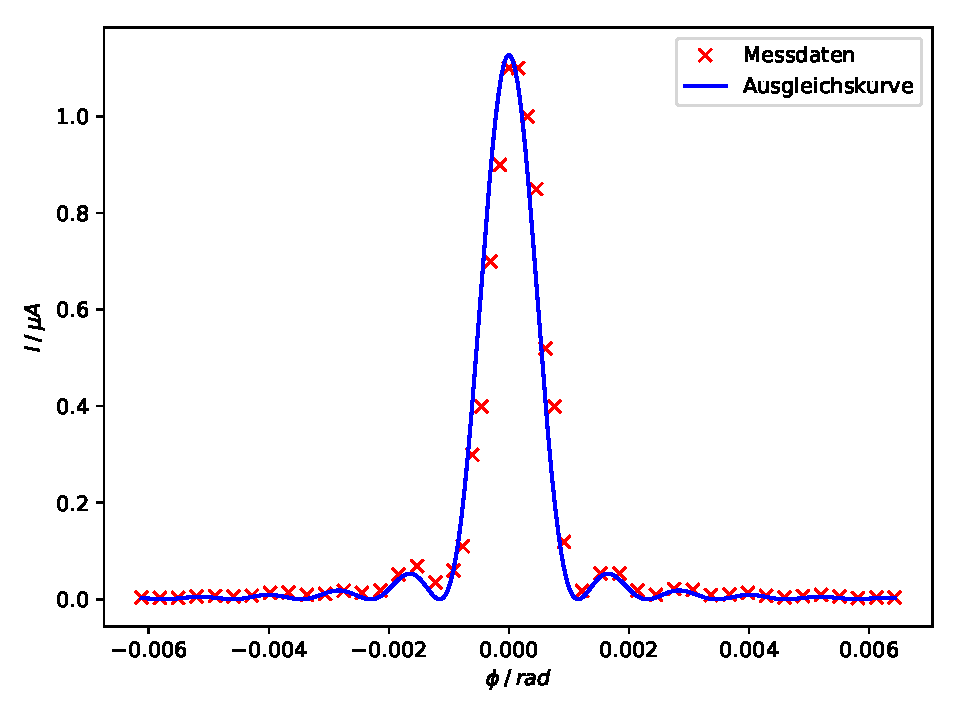
\includegraphics{content/plot1.pdf}
  \caption{Beugungsmuster des Einfachspaltes mit Spaltbreite $b = \SI{0.15}{\milli\meter}$}
  \label{fig:plot1}
\end{figure}

%2222222222222222222222222222222222222222222222222222222222222222222222222222222222222222222222

\subsection{Der Einfachspalt der Spaltbreite $b = \SI{0.075}{\milli\meter}$}

Die Messwerte des zweiten Einzelspalts sind in Tabelle \ref{tab:mess2} aufgelistet.
Auch hier sind die Messwerte und der Fit mittels python nach Form der Gleichung \eqref{eqn:einfach}
in Abbildung \ref{fig:plot2} abgebildet.

\begin{table}
        \centering
        \caption{Gemessenes Beugungsmuster des Einfachspaltes mit Spaltbreite $b = \SI{0.075}{\milli\meter}$}
        \label{tab:mess2}
        \sisetup{table-format=2.1}
        \begin{tabular}{c c c c c}
        \toprule
        $ l \;/\; \si{\milli\meter} $ & $I \;/\; \si{\micro\ampere}$ & &
        $ l \;/\; \si{\milli\meter} $ & $I \;/\; \si{\micro\ampere}$ \\
        \midrule 
        -25,0 & 0,0012 & \; &  1,0 & 0,3000 \\
        -24,0 & 0,0012 & \; &  2,0 & 0,2300 \\
        -23,0 & 0,0012 & \; &  3,0 & 0,1600 \\
        -22,0 & 0,0013 & \; &  4,0 & 0,0850 \\
        -21,0 & 0,0017 & \; &  5,0 & 0,0360 \\
        -20,0 & 0,0023 & \; &  6,0 & 0,0120 \\
        -19,0 & 0,0030 & \; &  7,0 & 0,0080 \\
        -18,0 & 0,0035 & \; &  8,0 & 0,0140 \\
        -17,0 & 0,0037 & \; &  9,0 & 0,0200 \\
        -16,0 & 0,0040 & \; & 10,0 & 0,0220 \\
        -15,0 & 0,0045 & \; & 11,0 & 0,0170 \\
        -14,0 & 0,0060 & \; & 12,0 & 0,0100 \\
        -13,0 & 0,0090 & \; & 13,0 & 0,0050 \\
        -12,0 & 0,0120 & \; & 14,0 & 0,0040 \\
        -11,0 & 0,0130 & \; & 15,0 & 0,0060 \\
        -10,0 & 0,0125 & \; & 16,0 & 0,0080 \\
         -9,0 & 0,0100 & \; & 17,0 & 0,0090 \\
         -8,0 & 0,0080 & \; & 18,0 & 0,0080 \\
         -7,0 & 0,0140 & \; & 19,0 & 0,0050 \\
         -6,0 & 0,0370 & \; & 20,0 & 0,0025 \\
         -5,0 & 0,0820 & \; & 21,0 & 0,0015 \\
         -4,0 & 0,1600 & \; & 22,0 & 0,0020 \\
         -3,0 & 0,2200 & \; & 23,0 & 0,0025 \\
         -2,0 & 0,2900 & \; & 24,0 & 0,0035 \\
         -1,0 & 0,3400 & \; & 25,0 & 0,0035 \\
          0,0 & 0,3500 & \; & &  \\
        \bottomrule
        \end{tabular}
    \end{table}

Es ergeben sich die Parameter 

\begin{align*}
    A_0 &= \SI{2460.41 +- 1297878.80}{\ampere\per\meter} \\
    b &= \SI{0.2 +- 127.7}{\milli\meter} \; .
\end{align*}

Der relative Fehler der gemessenen zur tatsächlichen Spaltbreite beträgt $\SI{166.66}{\percent}$.

\begin{figure}
    \centering
    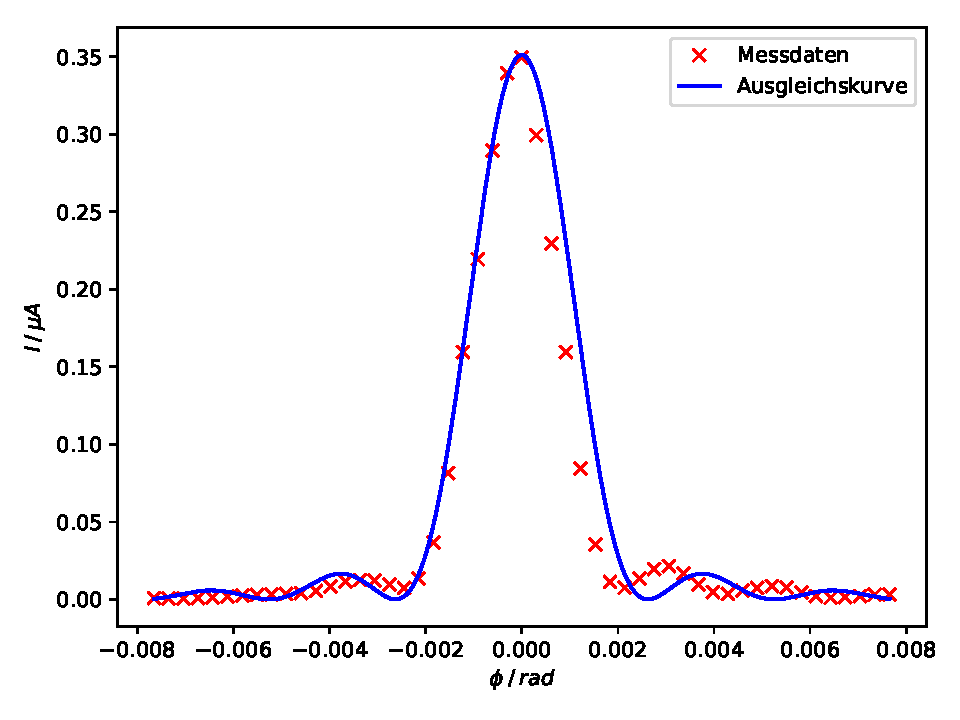
\includegraphics{content/plot2.pdf}
    \caption{Beugungsmuster des Einfachspaltes mit Spaltbreite $b = \SI{0.075}{\milli\meter}$}
    \label{fig:plot2}
  \end{figure}


%3333333333333333333333333333333333333333333333333333333333333333333333333333333333333333333333333333

\subsection{Der Doppelspalt}

Für den Doppelspalt mit Spaltbreite $b = \SI{0.15}{\milli\meter}$ und Spaltabstand
$s = \SI{0.1}{\milli\meter}$ sind die Messwerte in Tabelle \ref{tab:mess3} aufgelistet.


\begin{table}
            \centering
            \caption{Gemessenes Beugungsmuster des Doppelspalts}
            \label{tab:mess3}
            \sisetup{table-format=2.1}
            \begin{tabular}{c c c c c}
            \toprule
            $ l \;/\; \si{\milli\meter} $ & $I \;/\; \si{\micro\ampere}$ & &
            $ l \;/\; \si{\milli\meter} $ & $I \;/\; \si{\micro\ampere}$ \\
            \midrule 
            -25,0 & 0,0076 & \; &  1,0 & 0,0400 \\
            -24,0 & 0,0110 & \; &  2,0 & 0,0054 \\
            -23,0 & 0,0079 & \; &  3,0 & 0,0092 \\
            -22,0 & 0,0030 & \; &  4,0 & 0,0430 \\
            -21,0 & 0,0013 & \; &  5,0 & 0,0680 \\
            -20,0 & 0,0083 & \; &  6,0 & 0,0610 \\
            -19,0 & 0,0200 & \; &  7,0 & 0,0290 \\
            -18,0 & 0,0260 & \; &  8,0 & 0,0038 \\
            -17,0 & 0,0190 & \; &  9,0 & 0,0092 \\
            -16,0 & 0,0052 & \; & 10,0 & 0,0360 \\
            -15,0 & 0,0028 & \; & 11,0 & 0,0520 \\
            -14,0 & 0,0200 & \; & 12,0 & 0,0420 \\
            -13,0 & 0,0440 & \; & 13,0 & 0,0175 \\
            -12,0 & 0,0490 & \; & 14,0 & 0,0021 \\
            -11,0 & 0,0300 & \; & 15,0 & 0,0063 \\
            -10,0 & 0,0061 & \; & 16,0 & 0,0210 \\
             -9,0 & 0,0058 & \; & 17,0 & 0,0270 \\
             -8,0 & 0,0340 & \; & 18,0 & 0,0020 \\
             -7,0 & 0,0635 & \; & 19,0 & 0,0074 \\
             -6,0 & 0,0635 & \; & 20,0 & 0,0010 \\
             -5,0 & 0,0340 & \; & 21,0 & 0,0037 \\
             -4,0 & 0,0054 & \; & 22,0 & 0,0094 \\
             -3,0 & 0,0088 & \; & 23,0 & 0,0110 \\
             -2,0 & 0,0410 & \; & 24,0 & 0,0072 \\
             -1,0 & 0,1400 & \; & 25,0 & 0,0028 \\
            \bottomrule
            \end{tabular}
    \end{table}

Der Fit mittels python nach der Formel \eqref{eqn:doppel} ist zusammen mit den Messwerten in Abbildung
\ref{fig:plot3} aufgetragen.

Die Parameter sind:

\begin{align*}
    A_0 &= \SI{0.37 +- 35.07}{\ampere} \\
    b &= \SI{0.1 +- 1031.1}{\milli\meter} \\
    s &= \SI{0.4 +- 834.9}{\milli\meter} \; .
\end{align*}

Die relativen Fehler der Spaltbreite $b$ und des Spaltabstandes $s$ betragen $\SI{33.33}{\percent}$
und  $\SI{300}{\percent}$.

Das Beugungsmuster des Doppelspaltes unterscheidet sich von dem des ersten Einfachspaltes darin,
dass:

\begin{itemize}
    \item das Hauptmaximum des Doppelspaltes von etwa $\SI{0.14}{\micro\ampere}$ fast zehnfach
    kleiner als das des Einzelspaltes mit $\SI{1.2}{\micro\ampere}$ ist.
    \item das Hauptmaximum des Doppeltspaltes nicht um so viel größer als seine Nebenmaxima ist,
    wie das des Einzelspaltes.
    \item die Breite des Beugungsbildes des Doppelspaltes größer als die des Einzelspaltes ist.
\end{itemize}

\begin{figure}
    \centering
    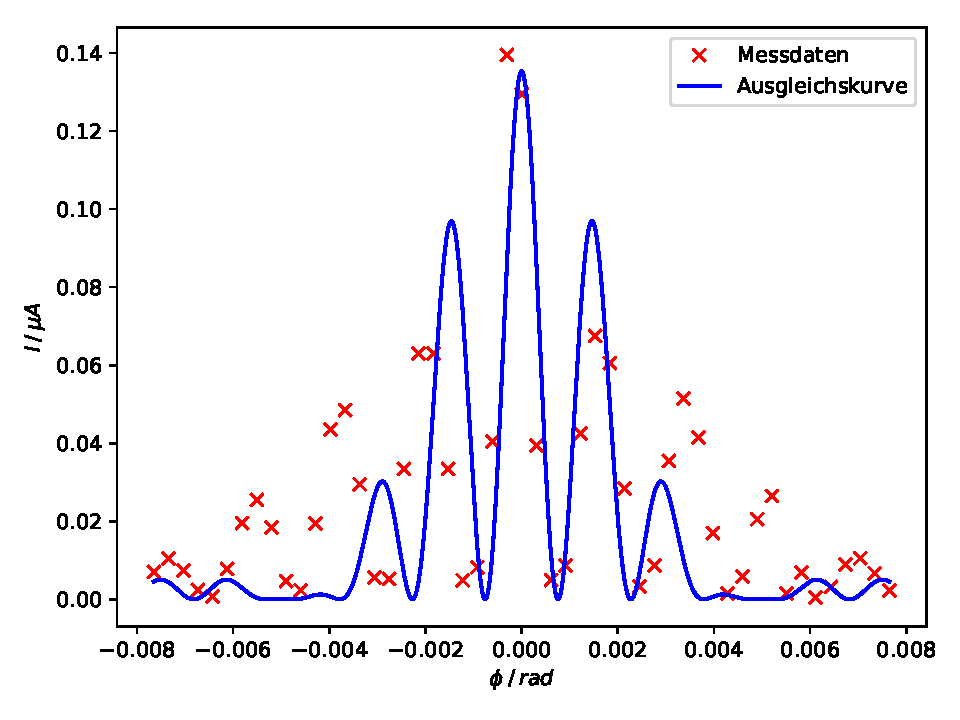
\includegraphics{content/plot3.pdf}
    \caption{Beugungsmuster des Doppelspaltes}
    \label{fig:plot3}
  \end{figure}


